% !TeX spellcheck = it_IT
% !TEX encoding = utf8
% !TEX root = main.tex

\chapter{Cédric Villani: il teorema vivente}
Matematico francese, 43 anni, attivo nel campo delle equazioni differenziali e della fisica matematica, conosciuto per il suo look fatto di cravatte da dandy, panciotti con orologio nel taschino e una spilla a forma di ragno sul bavero della giacca. Ma chi é Cédric Villani?! Come mai tutti ne parlano?
\section{Biografia}
\marginpar{
	\captionsetup{type=figure}
	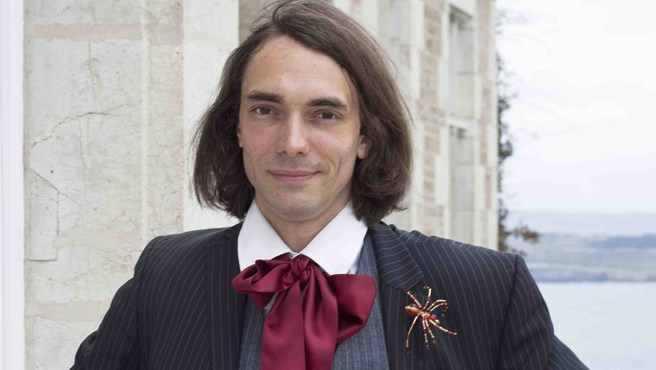
\includegraphics[width=\marginparwidth]{villani.jpg}
	\caption{Cédric Villani}
	\label{fig:villani}
}

Cèdric Villani compie i suoi studi all’\emph{École Normale Superiore} a Parigi (la sorella maggiore della \emph{Scuola Normale} di Pisa, per intenderci, nonchè uno degli istituti più importanti dell’intera Europa) dal 1992 al 1996, dove diventa anche \emph{assistant professor}. Nel 2000 si trasferisce a Lione, dove ottiene la cattedra e lavora tuttora, mentre dal 2009 è anche direttore dell’isituto Poincaré.
Sempre nel 2009 riceve la Medaglia Fermat mentre nel 2010 riceve la Medaglia Fields. Ha solo 37 anni.

Nel 2012 esce il suo celebre libro \emph{\textbf{Théorème vivant}} (il \emph{Teorema vivente}, edito da Rizzoli) nel quale spiega il suo lavoro e cosa vuol dire fare ricerca nel ramo della matematica. Nel 2016 è protagonista del TED talk di Vancouver mentre dal 2016 è un parlamentare della legislazione Macron.

\section{Vita privata e celebrità}
Cédric Villani è considerato un personaggio curioso per il suo aspetto e le sue passioni (divora fumetti manga giapponesi), dotato di un intuito fuori dal comune. Un genio della matematica, un vero ninja, in grado però di spiegare anche i temi più complessi con parole semplici e al grande pubblico. In molti lo hanno conosciuto con la pubblicazione del già citato saggio «Il Teorema vivente. La mia più grande avventura matematica».

Ma cosa fa dunque Cédric Villani? Ebbene i suoi studi riguardano la teoria delle equazioni differenziali alle derivate parziali coinvolte nella meccanica statistica; in particolare sull’equazione di Boltzmann, sulla quale ha vinto la celebre Medaglia. Ha lavorato inoltre sulla teoria del trasporto ottimale e sulle sue applicazioni in geometria differenziale. So che alcuni di voi potrebbero essersi persi, però il tempo di un caffè non è sufficiente per dilungarsi su cosa vertano questi argomenti. Per conoscenza però vi dico solo che sono alcuni degli argomenti più “caldi” della fisica matematica moderna.
\section{Il sogno della «città della scienza»}

A qualcuno leggendo le prossime righe potrebbe tornare in mente Platone e la sua idea della società perfetta guidata dai filosofi… ma vediamo perchè

Nelle ultime elezioni legislative francesi è stato candidato per il dipartimento francese della regione dell’Ile-de-France (Francia sud, per capirci, dove ci sono Lione, Grenoble e Saclay). Proprio là dove si trova la città di Saclay, considerata la Silicon Valley alla francese, e dove Villani avrebbe il desiderio di creare una cittadella della scienza e della tecnologia. Questo progetto è da molti considerato quasi utopico, ma se ci crede una Medaglia Fields, merita di farci un pensierino…

Spero con queste poche righe di avere suscitato in voi l’interesse per questa eclettica persona dagli interessi più svariati. Per approfindimento ti consiglio l'intervista sul sito di Madmaths citata nella Bibliografia \cite{url:maddmath_villani}! Attualmente in Francia è considerato come una celebrità e di sicuro se ne sentirà ancora parlare di lui.